\section{Behavior Design Patterns}

% Two columns start
\iftwocolumns
\begin{multicols}{2}
\fi

The behavior design patterns recognizes the problem in common software developments and provided more flexible communication between classes and class hiearchies. The overall benefits are more robust and flexible software.

\subsection{Command}\label{ssection:command}

The command design pattern decouples action request and action handlers. The callee who makes the request makes no assumptions about the class the receives the command. The decoupling between the two classes means that the client does not know anything about the handler. Likewise, the handler does not know anything about the callee of the command.\bs
\\
A loosely related real life analogy would be managers and programmers. Suppose programmer are specialized and can code a specific kind of software, and the managers tell programmers what to make. In a tightly coupled, without utilizing the command pattern, the manager is specialized too. Different programmer would need a different manager and the specific ``manager-to-programmer'' mapping cannot get broken (i.e. it does not make sense to have a manager responsible for online-services to give tasks to a graphics programmer).\bs
\\
Using the command pattern, the manager makes no assumption about who will be assigned the task/command they request. The manager simply broadcasts its requests out and moves on. Similarly, the programmer (handler) makes no assumption on who issued the task/command. But if the programmer is responsible for that type of task/command, they will perform the corresponding action.\bs
\\
In video games, the command pattern is most applicable in input mapping. An input is any input player gives to the game, such as controller axis and buttons, mouse presses, mouse move, and keyboard key pressed. In a tightly coupled scenario, the video game features a single control scheme and the player cannot customize it. Many older video games such as Tetris\cite{nes-tetris} and Super Mario Bros \cite{nes-mario} feature relatively simple controls. In addition to the limitation of the hardware which hinders the flexibility of the software, there is no customizable input mapping.\bs
\\
In nearly all of the newer game titles, regardless of they are from AAA production or independent developers, remappable inputs are almost an industry standard. Quality assurance (QA) of game studios rigorously perform compliance testing to ensure that remappable inputs function for customization as well as accessbility to increase player satisfaction.\bs
\\
In the example shown in figure \ref{fig:csgo-input}\cite{csgo-input}, the game Counter-Strike: Global Offensive (CSGO) by Valve demonstrates remappable inputs which is a convention adopted by the video game industry.

\begin{figure}[H]
	\centering
	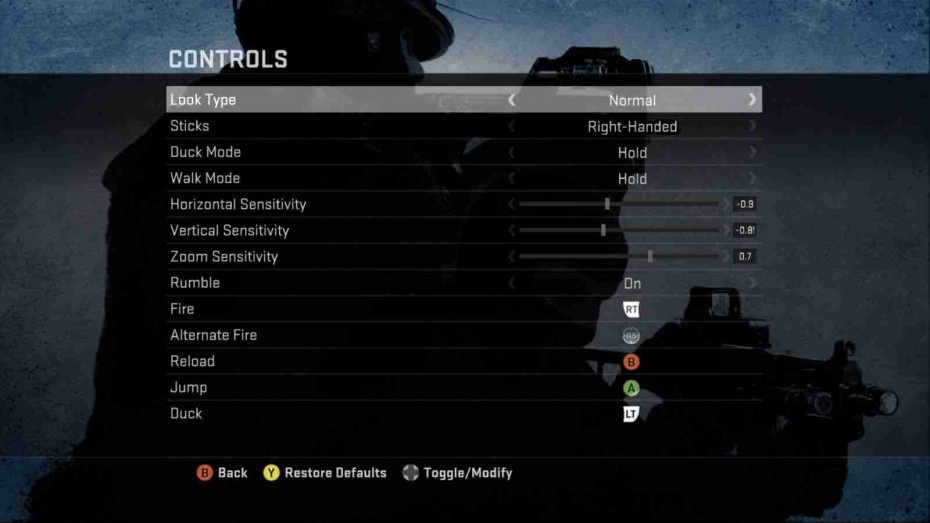
\includegraphics[width=\fullwidth]{assets/csgo-inputs}
	\caption{Option menus for optional input remapping in the CSGO}
	\label{fig:csgo-input}
\end{figure}

On the left side, we have the description of what handler a particular input would be attached to (i.e. ``Fire'' action is bounded to the controller's \textit{right trigger} button). By selecting this menu item and apply a new input, we could remap the action \textit{fire} to something else. This is extremely useful if the player does not own a controller, has disabilities that prevent them from reaching certain inputs, or just prefers their own input scheme. Note that CSGO is not special and is presented for the sake of the example. Modern games (especially ones that shipped to PC) will most certainly feature remappable inputs.\bs
\\
The command design pattern opens up more flexibility in mapping a requests to a handler. The software programming as well as game design is opened to be flexible. The callee invokes a command object that holds a reference to the \textit{real object} so that the handler can be called. Note that the command object is a \textit{mediator} between the callee and the handler (see section \ref{ssection:mediator}). Thus, we are not limited to simply remapping inputs, other logic could be implemented in the layer between the callee and the handler. One instance is to also incorporate \textit{memento} design pattern and implement a simple undo/redo system.\bs
\\

\subsection{Chain of Responsibility}

In extension to \textit{commands} pattern, chain of responsiblity essentially maps a single command to multiple handlers in a chain. When a request is raised, the first handler in the chain will receive and the logic in the first handler can decide if it wants to ``lower'' or ``resolve'' the request. If resolves, the request will not be passed down the chain. Otherwise, the next handler will be called and the same request is passed.\bs
\\
A common real life example is the algorithm of giving someone money in exact amount, in cash. Because cash have some specific denominations, we build this chain of command where we first use the largest denomination and then move down the denominations. For example, if I need to pay \$255.60, the logic would look like this in figure \ref{fig:chain-pay}:

\begin{figure}[H]
	\centering

	\scalebox{0.75}{
		\begin{tikzpicture}
			\node (start)[startstop]{Start};
			\node (pay1)[process, below of=start]{Pay the difference in \$100};
			\node (calc1)[process, right of=pay1, xshift=4cm]{Recalculate difference};
			\node (pay2)[process, below of=pay1]{Pay the difference in \$50};
			\node (calc2)[process, right of=pay2, xshift=4cm]{Recalculate difference};
			\node (pay3)[process, below of=pay2]{Pay the difference in \$5};
			\node (calc3)[process, right of=pay3, xshift=4cm]{Recalculate difference};
			\node (pay4)[process, below of=pay3]{Pay the difference in \$0.25};
			\node (calc4)[process, right of=pay4, xshift=4cm]{Recalculate difference};
			\node (pay5)[process, below of=pay4]{Pay the difference in \$0.10};
			\node (end)[startstop, below of=pay5]{End};

			\draw [arrow](start)--(pay1);

			\draw [arrow](pay1)--(calc1);
			\draw [arrow](pay2)--(calc2);
			\draw [arrow](pay3)--(calc3);
			\draw [arrow](pay4)--(calc4);

			\draw [arrow](calc1)--(pay2);
			\draw [arrow](calc2)--(pay3);
			\draw [arrow](calc3)--(pay4);
			\draw [arrow](calc4)--(pay5);

			\draw [arrow](pay5)--(end);
		\end{tikzpicture}
	}

	\caption{Chain of Responsibility design pattern demonstrated in process of an real life scenario.}
	\label{fig:chain-pay}
\end{figure}

In video games, chain of responsiblity, in combination of the \textit{command} design pattern (section \ref{ssection:command}) are often used handle large scale UI. I will use the term \textbf{chain of commands} for the combined use of the two patterns.\bs
\\
In the Frostbite engine (and other game engines) there exists elements \textit{InputHandler} and \textit{InputDispatcher}. The input handler elemet utilizes the command pattern and on a high level, listens to a particular user input (mouse, keyboard, or controller) and outputs an event when the input is active. The input dispatcher element may hold references to other input handlers via links. This creates a chain of command as when an input is fired, the event travels up the chain of input handlers. Each input handler has some logic and could be customized to ``consume'' the input. Only the input handler that ``consumes'' the input will carry out the logic, and other input handlers down the chain will not receive the command.\bs
\\
The input dispatchers enable/disable input handlers on the chain. This is useful for when we only need certain inputs at certain time. For example, when in game, the mouse cursor is disabled as the player is using the mouse to control the camera, and the input for mouse buttons should correspond to aim and fire of the gun. However, when we activate menus, we show the cursor and disable the input to areas we just discussed. Instead turning on other UI related input handling such as mouse hover etc.\bs
\\

\begin{figure}[H]
	\centering
	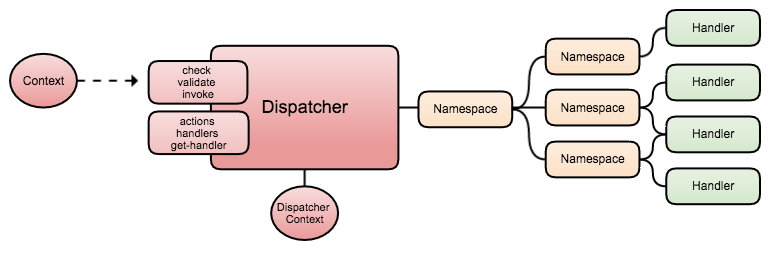
\includegraphics[width=\fullwidth]{assets/inputdispatch}
	\caption{General model of input tree with input handlers and input dispatchers}
	\label{fig:inputdispatch}
\end{figure}

During handling of mouse press when there are multiple \textit{hitzones}\footnote{Hitzones are interactive areas for mouse that reports data and events such as mouse position, if mouse is hover, mouse button presses and releases} overlapped (figure \ref{fig:chainofcommand-mousezones}). Any press or hovering event will be handled by the top-most hitzone entity first. If the handler does not consume the input event, the event will naturally "flow" down to the next level.
\bs

\begin{figure}[H]
	\centering
	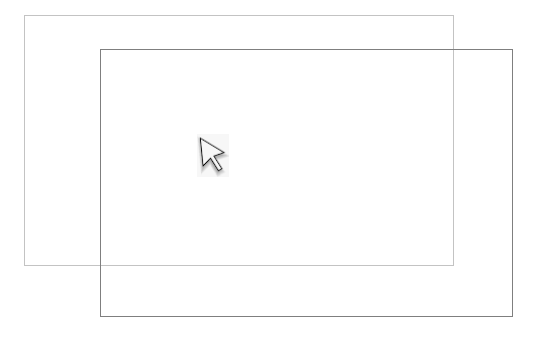
\includegraphics[width=0.3\textwidth]{assets/mousehover}
	\caption{Mouse interacting with overlapping mouse hitzones}
	\label{fig:chainofcommand-mousezones}
\end{figure}

\subsection{Mediator}\label{ssection:mediator}

% TODO:

Mediator acts as a middle-man between communicating objects and decouples them\cite{sm-mediator}.

\begin{figure}[H]
	\centering
	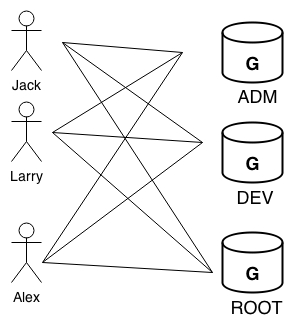
\includegraphics[width=0.3\textwidth]{assets/mediator_before}
	\caption{Objects communicating without using mediator pattern}
	\label{fig:mediator-before}
\end{figure}

\begin{figure}[H]
	\centering
	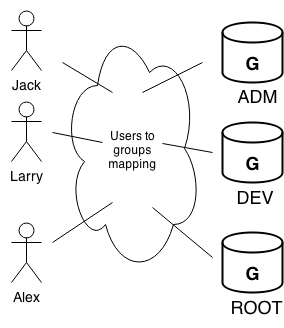
\includegraphics[width=0.3\textwidth]{assets/mediator_after}
	\caption{Objects communicating using mediator pattern}
	\label{fig:mediator-after}
\end{figure}

As seen in figure \ref{fig:mediator-before}, complexity of interactions between objects become exponentially large as the software grows.\bs
\\
Such problem occurs often in UI: An example would be when a input signal is mapped to multiple elements. In particular, say we have a button to open up the game menu. Then at the same time there are a few systems we need to talk to during this. First, we need to tell the game to lock all inputs to the character in the world, so that when we're navigating the menu, we don't move the character around. We want to enable mouse cursor (and hide it during game play). We might want to pause the game so that enemies don't attack in the background while we have the menu open. We might want to optimize performance by turning off rendering of the world when we're in the menu, since we might not able to see it anyway.\bs
\\
Without using a mediator, the activated event from the button would need to invoke methods in all these different systems. This \textit{antipattern} breaks abstraction, tightly decouples all these systems together which makes it prone to error and crashes, and makes the code highly unmaintainable.\bs
\\
Instead, we use pattern as depicted in figure \ref{fig:mediator-after}. The button event should communicate with a middle-man that sets a state. The various systems that would be affected does not know anything about the button, or anything that interacts with the mediator. It merely gets the state stored in the mediator, and performs corresponding action.\bs
\\

% CHANGED: this may not be the case as shared lock is more of a 'critical system' solution
% In Frostbite, a similar mechanism is called a \textit{SharedLock}. 

\subsection{Memento}

Memento are design patterns for objects to know how to save and load (externalize) its own internal state and data.\bs
\\
Usability improvement: when used together with Command pattern, we can create undo/redo actions. Not as applicable in the game engine itself, but essential to the development tools and editors artists and scripters use to develop the game.\bs
\\

\textbf{Difference Between Command and Memento}\bs
\\

Command passes a request from the client to be handled while memento passes its own internal state. Using an analogy of how a player interacts in a game menu: a command would be the event of player clicking on the save/load buttons of their game files, and the memento would be the save file objects itself being saved/loaded.\bs
\\

\subsection{Observer}

The observer design pattern is ubiquitous to software development. Observers define a one-to-many dependency where many clients can ``subscribe'' to a state change of a particular object. The clients would be notified by the broadcast sent by the subscribed object.\bs
\\
In observer pattern, the object sending the events is the \textit{subject}, and the objects receiving are the \textit{observer}. The observer hierarchy consists of an abstract \textit{observer} base class, which has some handler (see figure \ref{fig:observer-simple}).

\begin{figure}[H]
	\centering

	\scalebox{0.75}{
		\begin{tikzpicture}
			\begin{class}[text width=8cm]{Subject}{0,0}
				\attribute{-observers: ObserverBase[]}
				\operation{+Subject():}
				\operation{+RegisterObserver(ObserverBase *observer):}
				\operation{+UnregisterObserver(ObserverBase *observer):}
				\operation{-fireEvent(...):}
			\end{class}

			\begin{interface}{ObserverBase}{0,-5}
				\operation[0]{+handleEvent(...);}
			\end{interface}

			\begin{class}{ConcreteObserver}{0, -8}
				\implement{ObserverBase}
				\operation{+handleEvent(...):}
			\end{class}

			\draw[->](Subject)--node[right, black]{$<<$broadcasts$>>$}(ObserverBase);
		\end{tikzpicture}
	}

	\caption{Simple subject-object relationship in observer design pattern}
	\label{fig:observer-simple}
\end{figure}

Without using any mediators, the subject is \textit{loosely coupled}\footnote{Loose coupling means dependency to another object via interface or abstract class. Whereas tight coupling means dependency to the concrete class directly.} to the observer types. The subject holds a collection or list of registered observers, such that when an event should be fired, the subject iterates through all the observers and deliver the event.\bs
\\
% The client is responsible for managing the observers' lifetime. The client or observers are responsible for when to register or unregister to a subject. In essence, the subject makes no assumption about its observers. (Similar to the relationship in model-view-controller where the controller act as observer to the view to enable user interaction - see section \ref{ssection:ecs}).\bs
\\
In Frostbite (and extends to many game engines and software), many OOP and inter-class relationship relies on events. A player's interaction with the controller, keyboard, or mouse triggers input events to be handled by the Input Handler. For example shown in figure \ref{fig:unreal-input}, the subject are objects that outputs an event whenever certain key is pressed (red blocks). The output event \textit{Released} is hooked up to some observer. The corresponding observers are the \textit{Move Updated Component} handlers that carries out specific tasks whenever it receives the event/signal.

\begin{figure}[H]
	\centering
	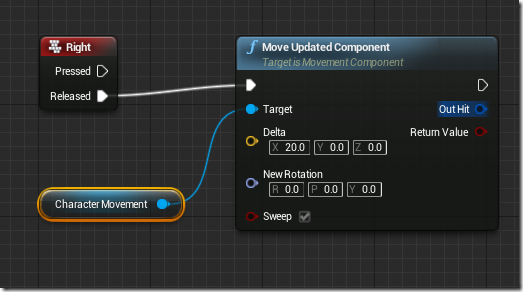
\includegraphics[width=0.49\textwidth]{assets/unreal-input}
	\caption{Example of event connections in Unreal Engine which is based on the observer design pattern. \cite{gfs-input}}
	\label{fig:unreal-input}
\end{figure}

It avoids the antipattern of \textit{spaghetti code} where increase in complexity of the software leads to exponential increase in complexity and unmaintainable code. The design pattern is very useful for organization, maintainability, flexibility, and scalability of code.\bs
\\
There are several approach to the implementation. Mainly, the subject could push data to observers during the function call. Or the observers could pull data from the subject. The observers could receive a subject pointer during construction and register themselves, or a client could register the observers for them. Nonetheless, the observer pattern is flexible and fit many needs in video game programming.\bs
\\
A sample code of an observer pattern example is in section \ref{code:observer}. In this example, we created a simple system to broadcast world events to a multiplayer game.

% \subsection{Visitor}
% TODO:


% Two columns end
\iftwocolumns
\end{multicols}
\fi